\documentclass[12pt,twoside]{article}
\usepackage{amsmath, amssymb}
\usepackage{amsmath}
\usepackage[active]{srcltx}
\usepackage{amssymb}
\usepackage{amscd}
\usepackage{makeidx}
\usepackage{amsthm}
\usepackage{algpseudocode}
\usepackage{algorithm}

\usepackage{fancyhdr}
\usepackage{graphics}
%----------------------------------------------------------------------------------------------
\usepackage{amsmath, amssymb}
\usepackage{amsmath}
\usepackage[active]{srcltx}
\usepackage{amssymb}
\usepackage{amscd}
\usepackage{makeidx}
\usepackage[dvips]{graphicx}
\usepackage{verbatim}

\renewcommand{\baselinestretch}{1}
\setcounter{page}{1}
\setlength{\textheight}{21.6cm}
\setlength{\textwidth}{14cm}
\setlength{\oddsidemargin}{1cm}
\setlength{\evensidemargin}{1cm}
\pagestyle{myheadings}
\thispagestyle{empty}
\markboth{\small{Pr\'actica 1. Le\'on Tejeda.}}{\small{.}}
\date{}
\begin{document}


\begin{figure}[h]
\vspace{-3cm} \hspace{-2cm} \setlength{\unitlength}{1mm}
\begin{comment}
\begin{picture}(15,25)(-10,0)
\includegraphics[width=16cm,height=3cm]{titulo.jpg}
\end{picture}
\end{comment}
\end{figure}


\vspace{0cm}

\centerline{\bf An\'alisis de Algoritmos, Sem: 2022-2, 3CV11, Pr\'actica 1, 02/03/2022}

\centerline{}

%\centerline{}


\begin{center}
\Large{\textsc{Pr\'actica 1: Determinaci\'on experimental de la complejidad temporal de un algoritmo}}
\end{center}
\centerline{}
\centerline{\bf {Tejeda Moyao Le\'on Francisco.}}
\centerline{}
\centerline{$leontejeda@gmail.com$}



\newtheorem{Theorem}{\quad Theorem}[section]

\newtheorem{Definition}[Theorem]{\quad Definition}

\newtheorem{Corollary}[Theorem]{\quad Corollary}

\newtheorem{Lemma}[Theorem]{\quad Lemma}

\newtheorem{Example}[Theorem]{\quad Example}

\bigskip

\textbf{Resumen:} Este programa realiza una comparaci\'on de datos entre sub arrelgos de tamaño n/2 para ver si se encuentran datos repetidos en dichos sub arreglos.




{\bf Palabras Clave:} Arreglos, Numeros Aleatorios, SubArreglos, Gr\'afica, C++.

\section{Introducci\'on}

Para poder entender lo que se est\'a haciendo en esta pr\'actica, primero definamos un algoritmo.

Un algoritmo se define como el conjunto ordenado y finito de operaciones que permite hallar la solución de un problema. Esto son bastante importante, ya que b\'asicamente la mayoría de las tareas que realiza una computadora se basan en algoritmos.

\textbf{¿Por qu\'e estudiarlos?}

La principal razón para estudiarlos es para saber cual es mas eficiente, puesto que, aunque 2 algoritmos pueden hacer la misma tarea, no significa que a ambos les tome el mismo tiempo realizar una tarea, esto tiene un impacto aun más grande cuando las cantidades de datos que se manejan son demasiado grandes.

\newpage


\section{Conceptos B\'asicos}
En esta practica graficaremos los puntos experimentales, independientemente si estos son los mejores o los peores casos.

\textbf{$\Theta$}: Son los puntos experimentales, lo que nuestro algoritmo encuentra.

\textbf{$O$} : Es el peor caso, que se da cuando nuestro algoritmo recorre todas las posiciones de ambos sub arreglos.

\textbf{$\Omega$}: es el mejor caso, que se da cuando nuestro algoritmo encuentra el numero repetido en el ultimo lugar de ambos sub arreglos.

Para la realización de esta practica hicimos uso de un algoritmo de búsqueda, el cual se fijará en el sub arreglo A1[n/2] y verificara si hay algún numero repetido en el arreglo A2[n/2], ambos sub arreglos salieron de un arreglo A[n] el cual está lleno de números aleatorios de 0 - 3N, el arreglo fue dividido en dos partes.

\medskip

\begin{figure}[h]
\vspace{3cm} \hspace{-2cm} \setlength{\unitlength}{1mm}
\begin{picture}(60,55)(-40,0)
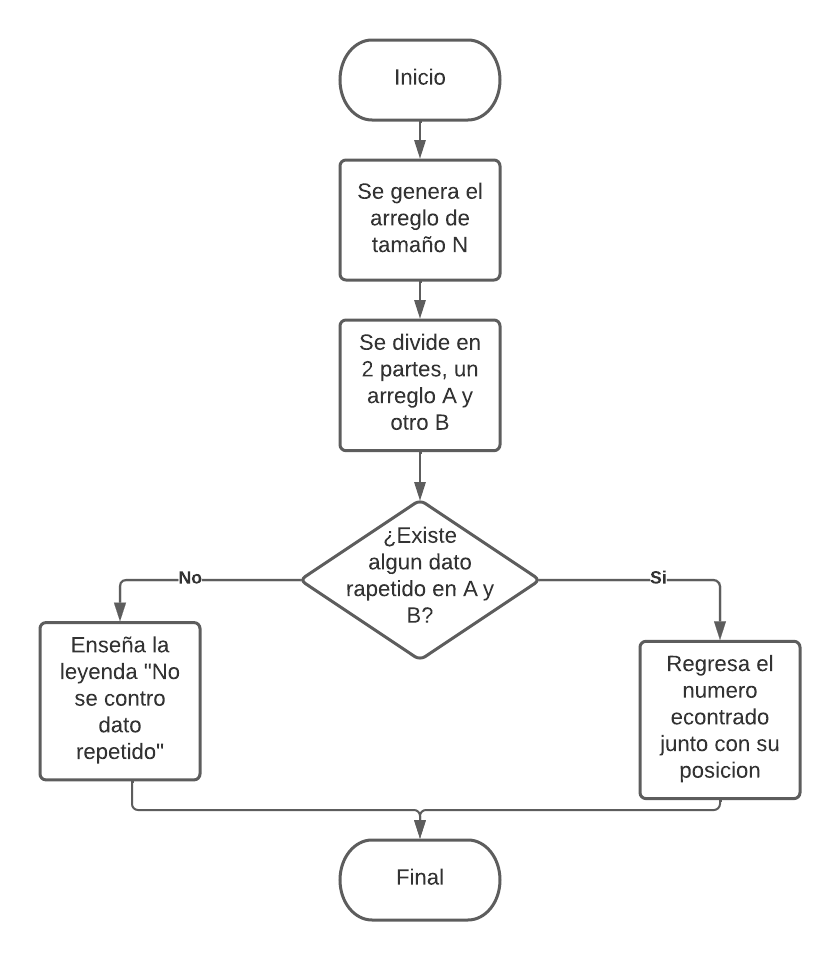
\includegraphics[width=9cm,height=9cm]{Diagrama.png}
\end{picture}
\end{figure}
\vspace{-1cm}
\begin{center}
Figura 1. Diagrama Flujo.
\end{center}
\medskip

\newpage

\section{Experimentaci\'on y Resultados}
El programa va a buscar en arreglos de tamaño 10, este va a aumentar de 10 en 10 hasta llegar a 1000, por lo que en la gráfica contaremos con 100 registros para así observar el comportamiento del algoritmo.
Nos basamos en el primer arreglo de 10 caracteres, podemos observar el comportamiento del algoritmo y por ende su resultado.

\begin{figure}[h]
\vspace{3cm} \hspace{-2cm} \setlength{\unitlength}{1mm}
\begin{picture}(10,10)(-50,-10)
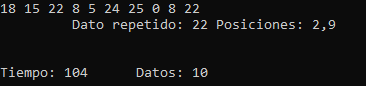
\includegraphics[width=7cm,height=3cm]{Arreglo10Si.png}
\end{picture}
\end{figure}
\vspace{-1cm}
\begin{center}
Figura 2. Arrelgo de tamaño 10 con coincidencia.
\end{center}
\medskip

\begin{figure}[h]
\vspace{3cm} \hspace{-2cm} \setlength{\unitlength}{1mm}
\begin{picture}(10,10)(-50,-10)
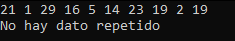
\includegraphics[width=7cm,height=2cm]{Arreglo10No.png}
\end{picture}
\end{figure}
\vspace{-1cm}
\begin{center}
Figura 3. Arrelgo de tamaño 10 sin coincidencia.
\end{center}
\medskip

\newpage

Al momento de graficar los puntos experimentales encontramos la siguiente imagen incluyendo las funciones por la cuales es acotada [G(n) y F(n)].
\begin{figure}[h]
\vspace{3cm} \hspace{-2cm} \setlength{\unitlength}{1mm}
\begin{picture}(50,55)(-40,-5)
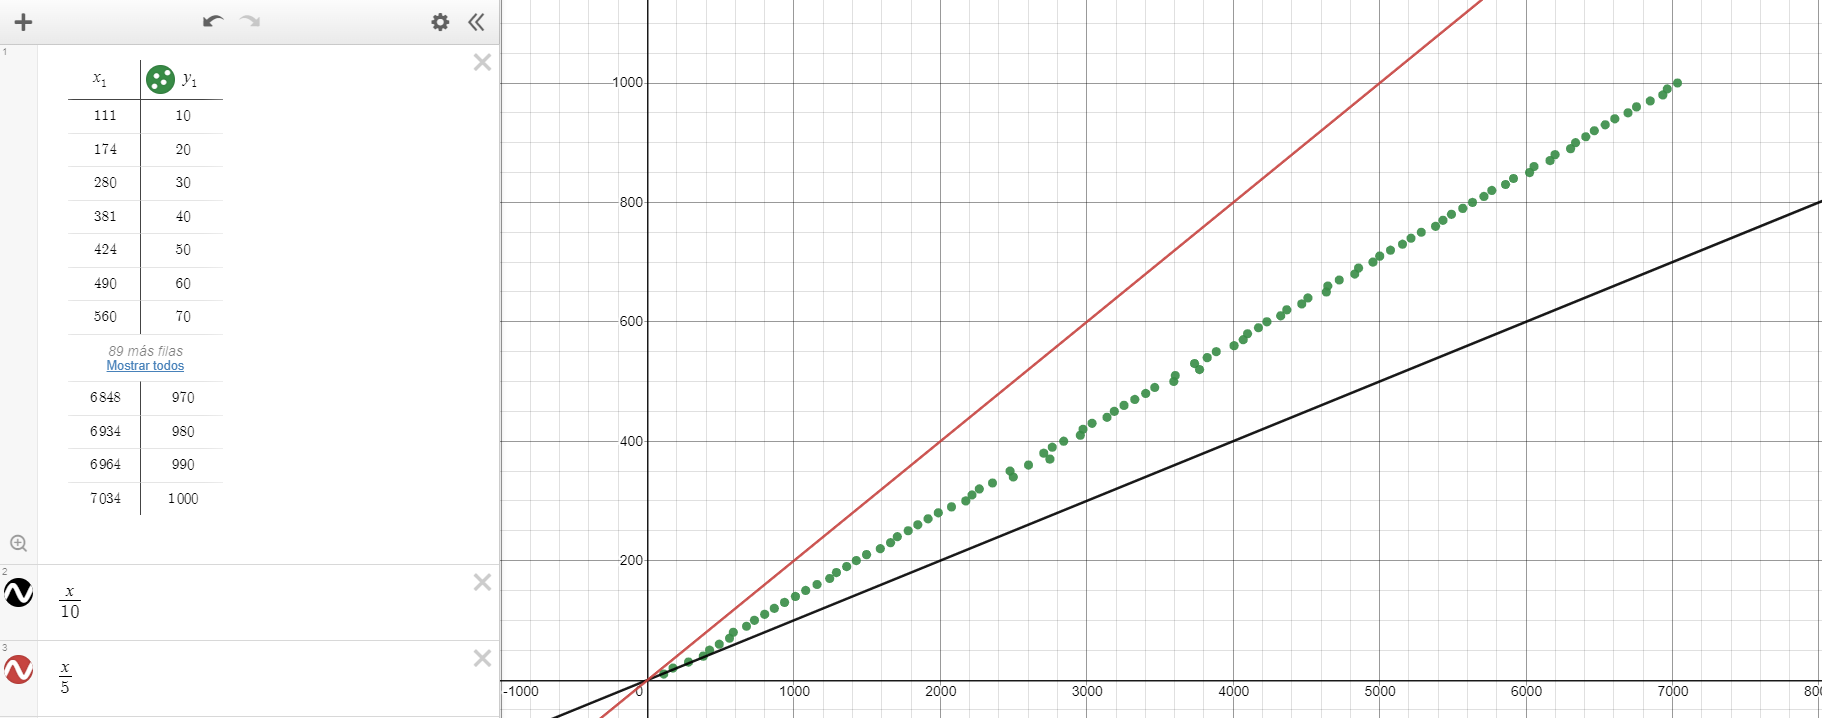
\includegraphics[width=10cm,height=8cm]{Grafica.png}
\end{picture}
\end{figure}
\vspace{-1cm}
\begin{center}
Figura 4. Gráfica con G(n) = x/5 y F(n)=x/10.
\end{center}
\medskip



\section{Conclusiones}
Leon Tejeda:

El análisis de algoritmos tiene un papel muy importante, ya que podríamos encontrar un método mucho más eficiente para resolver algún problema, también nos ayuda a ver si nuestra puede mejorar o no.
Aquí es  en donde mas tienen que ver las matemáticas, o donde más las vemos aplicadas, debido a que incluso se pueden ver series al momento de estar analizando algún código.
\begin{picture}(0,0)(-60,5)

\includegraphics[width=2.5cm,height=2.5cm]{Alumno.jpg}
\end{picture}

\end{document}
